\section{Political Case Studies}

\subsection{The Subreddits}
Currently I have 8 case study politically-oriented subreddits. There are loosely ordered from most politically right wing to most left wing, with quoted community description:

\begin{enumerate}
    \item \href{https://www.reddit.com/r/The_Donald}{r/The\_Donald: ``The\_Donald is a never-ending rally dedicated to the 45th President of the United States, Donald J. Trump."}
    
    \item \href{https://www.reddit.com/r/Libertarian}{r/Libertarian: ``A place to discuss free market libertarianism and related topics, and share things that would be of interest to libertarians.''}
    
    \item \href{https://www.reddit.com/r/Conservative}{r/Conservative: ``The place for Conservatives on Reddit." }
    
    \item \href{https://www.reddit.com/r/politics}{r/politics: ``/r/Politics is for news and discussion about U.S. politics."}
    
    \item \href{https://www.reddit.com/r/Conservative}{r/changemyview: ``A place to post an opinion you accept may be flawed, in an effort to understand other perspectives on the issue. Enter with a mindset for conversation, not debate."}
    
    \item \href{https://www.reddit.com/r/socialism}{r/socialism: ``This is a community to discuss current events in our world from an anti-capitalist perspective and to provide clarity to socialist ideas"}
    \item \href{https://www.reddit.com/r/SandersForPresident}{r/SandersForPresident: ``Run Bernie Run!"}
    \item \href{https://www.reddit.com/r/LateStageCapitalism}{r/LateStageCaptialism: ``A One-Stop-Shop for Evidence of our Social, Moral and Ideological Rot.''}
\end{enumerate}

Both r/The\_Donald and r/LateStageCapitalism clearly state that they will remove content and ban users who dissent from their respective general opinions, i.e. Pro-Trump or anti-capitalist sentiment. As such they can be considered to tacitly encourage echo chamber behaviours. At this point I take them to be my examples of a right wing and a left wing echo chamber. r/politics is the only default subreddit on the list. It is a place for general discussions on US politics, with no set political stance, thus I've place it in the middle of the list. r/changemyview was created to be an "anti-echo chamber", to actively encourage people with opposing opinions to debate each other. I therefore place it in the middle of the list. The r/Libertarian, r/Conservative, and r/socialism are all generalist subreddits which each favour their named viewpoints. r/SandersforPresident was originally inteded to supporter Bernie Sander's run for the US Presidency in 2016. It is fairly active, and likely to see a resurgence heading into 2020.

\subsection{Findings}

% Political Visuals
\begin{figure}
    \centering
    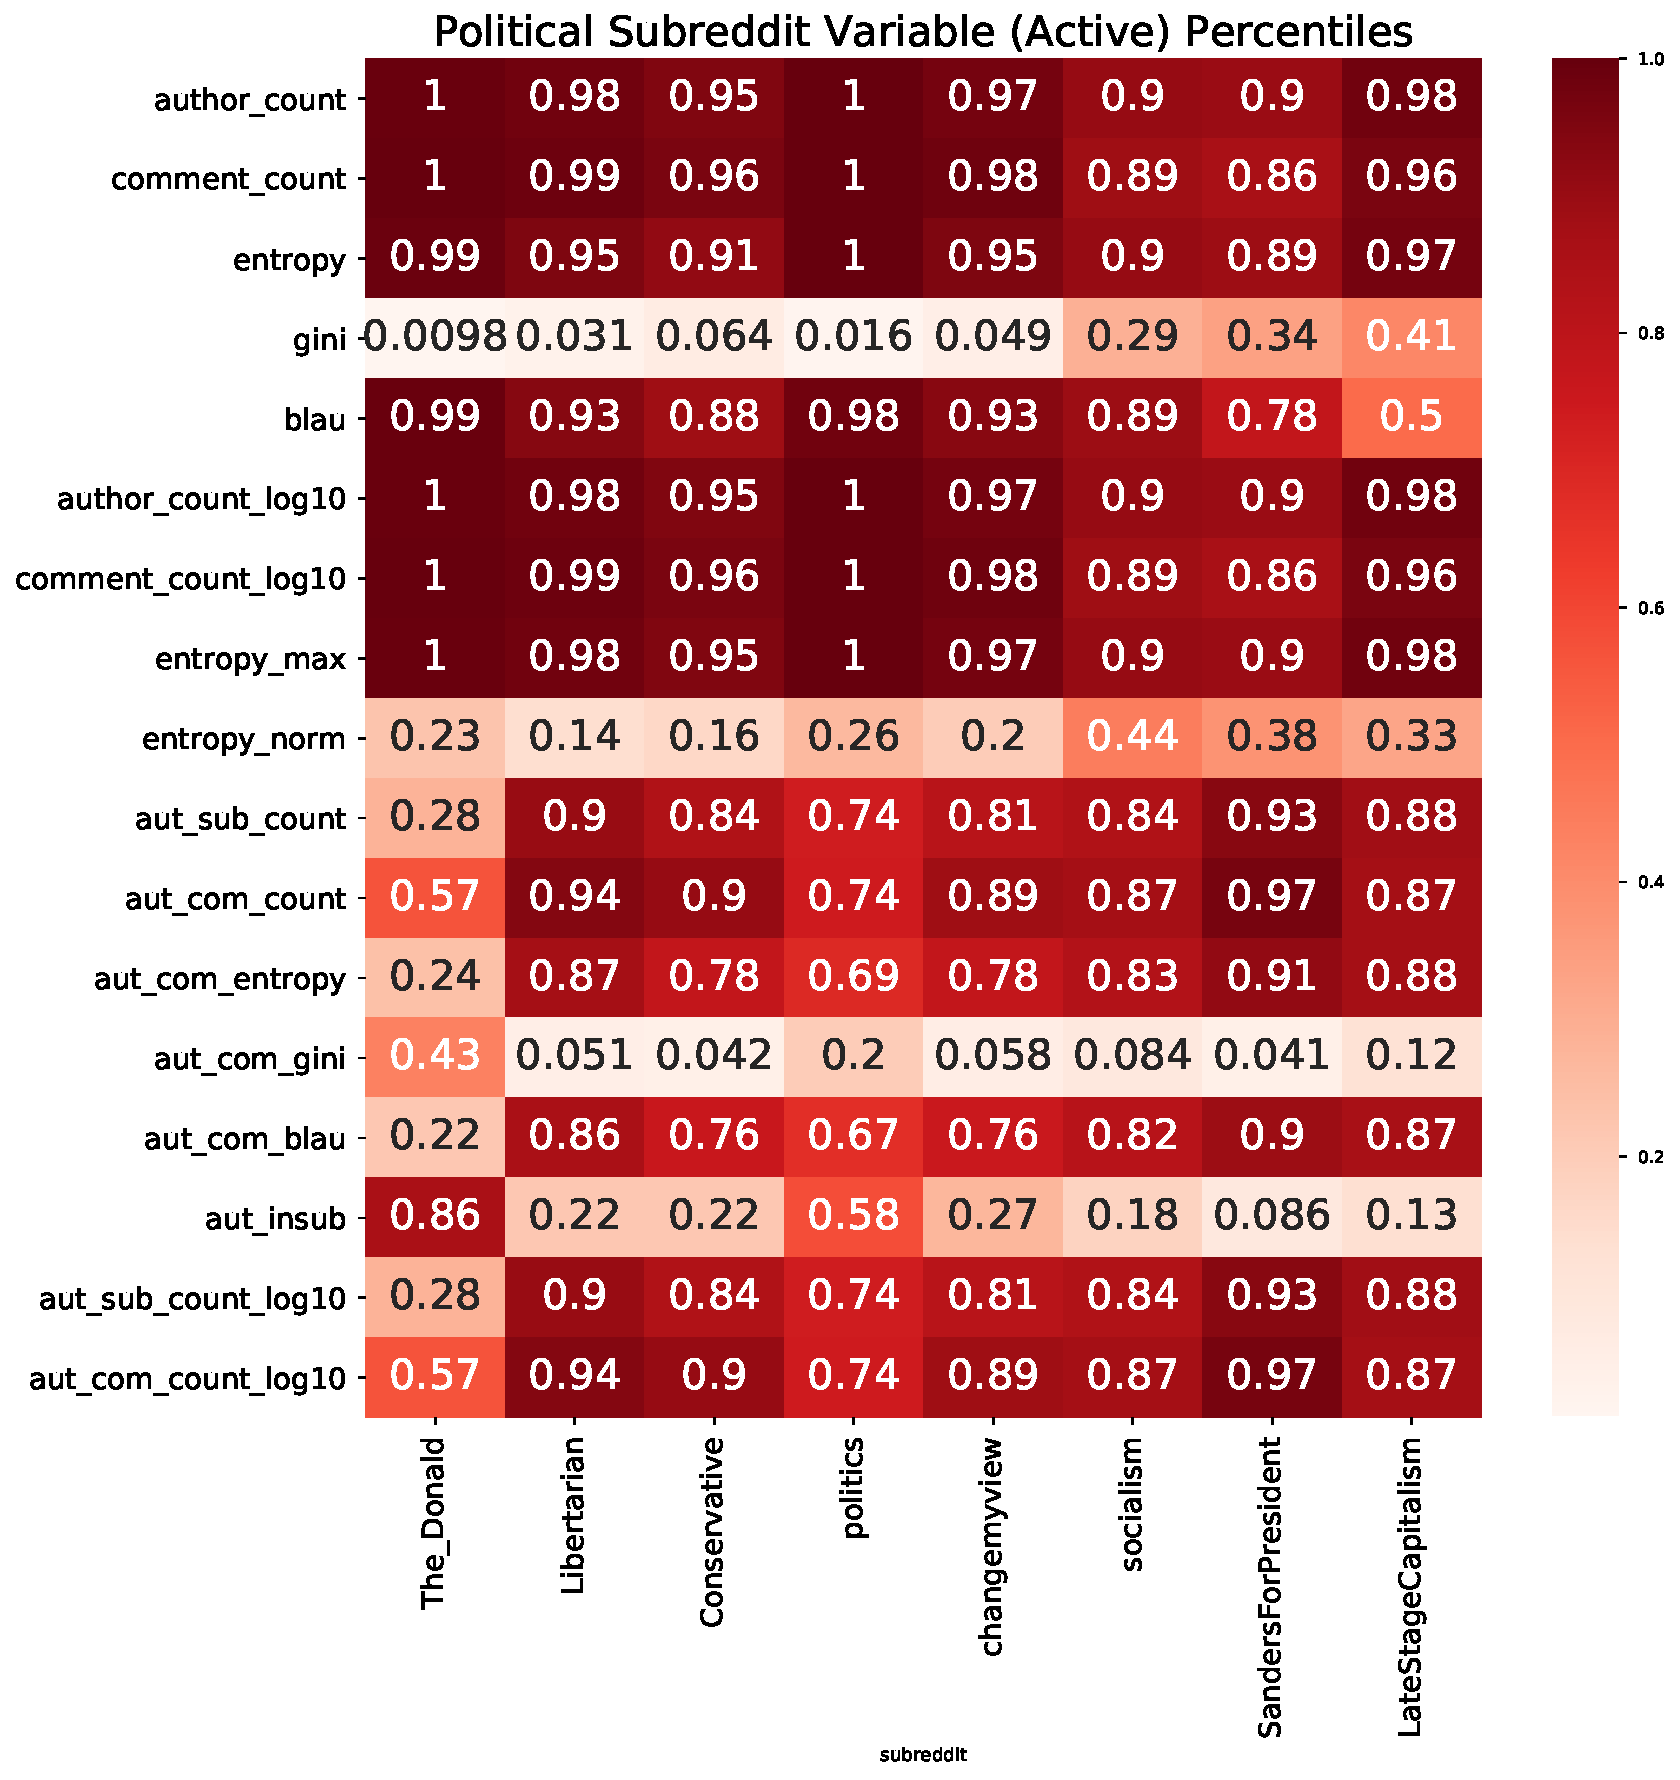
\includegraphics[scale=0.5]{latex/pol-heatmap.pdf}
    \caption{Political Subreddit Variable Percentiles}
    \label{pol-heatmap}
\end{figure}


\begin{landscape}
\begin{table}
\centering
\begin{tabular}{lrrrrrrrr}
\toprule
subreddit &  The\_Donald &  Libertarian &  Conservative &   politics &  changemyview &  socialism &  SandersForPresident &  LateStageCapitalism \\
\midrule
author\_count        &    44917.00 &     13249.00 &       6468.00 &  136116.00 &      11215.00 &    3664.00 &              3445.00 &             15091.00 \\
comment\_count       &   784104.00 &    107933.00 &      42927.00 & 1624275.00 &      86088.00 &   13777.00 &             11509.00 &             43005.00 \\
entropy             &        9.20 &         7.95 &          7.41 &      10.21 &          7.95 &       7.30 &                 7.18 &                 8.41 \\
gini                &        0.20 &         0.25 &          0.28 &       0.22 &          0.26 &       0.39 &                 0.41 &                 0.44 \\
blau                &        1.00 &         1.00 &          1.00 &       1.00 &          1.00 &       1.00 &                 1.00 &                 0.99 \\
author\_count\_log10  &        4.65 &         4.12 &          3.81 &       5.13 &          4.05 &       3.56 &                 3.54 &                 4.18 \\
comment\_count\_log10 &        5.89 &         5.03 &          4.63 &       6.21 &          4.93 &       4.14 &                 4.06 &                 4.63 \\
entropy\_max         &       10.71 &         9.49 &          8.77 &      11.82 &          9.33 &       8.21 &                 8.14 &                 9.62 \\
entropy\_norm        &        0.86 &         0.84 &          0.84 &       0.86 &          0.85 &       0.89 &                 0.88 &                 0.87 \\
aut\_sub\_count       &        5.00 &        16.00 &         13.00 &      10.00 &         12.00 &      13.00 &                18.00 &                15.00 \\
aut\_com\_count       &       22.00 &        57.00 &         50.00 &      31.00 &         47.00 &      45.00 &                66.00 &                45.00 \\
aut\_com\_entropy     &        1.21 &         2.18 &          1.94 &       1.75 &          1.93 &       2.06 &                 2.30 &                 2.18 \\
aut\_com\_gini        &        0.64 &         0.53 &          0.53 &       0.59 &          0.54 &       0.55 &                 0.53 &                 0.57 \\
aut\_com\_blau        &        0.62 &         0.83 &          0.80 &       0.77 &          0.80 &       0.82 &                 0.85 &                 0.84 \\
aut\_insub           &        0.27 &         0.05 &          0.05 &       0.13 &          0.06 &       0.05 &                 0.03 &                 0.04 \\
aut\_sub\_count\_log10 &        0.70 &         1.20 &          1.11 &       1.00 &          1.08 &       1.11 &                 1.26 &                 1.18 \\
aut\_com\_count\_log10 &        1.34 &         1.76 &          1.70 &       1.49 &          1.67 &       1.65 &                 1.82 &                 1.65 \\
\bottomrule
\end{tabular}
\caption{Political Subreddit Results}
\label{table/pol}
\end{table}
\end{landscape}

\subsubsection{Size}
The subreddits list so far we selected from a manual search of the 500 (or 1000?) most active subreddits during a previous sampling stage. This list can be easily extended as more appropriate politically-oriented subreddits come to my attention.

Figure \ref{pol-heatmap} shows the percentiles for  these political subreddits, compared to the 8094 active subreddits. The raw data can bee seen in Table \ref{table/pol}. All of the subreddits are the in 90th or higher percentile by author count, and 96th percentile for comment count (with the exception of r/socialism (89th) and r/SandersForPresident (86th). 

\subsubsection{Diversity}
All of the subreddits have a gini value lower than the median for active subreddits. The three left wing subreddits have low to middle values (29th, 34th, and 41st percentiles). These correspond to gini values of 0.39, 0.41, and 0.44. The remaining 5 subreddits are all in the lowest 5\% of subreddits by gini. These values range from 0.2 to 0.26. 

All subreddits are in 89th or higher percentile for entropy. Most of the subreddits are in the 89th or higher percentile for blau. r/SandersForPresident and r/LateStageCapitalism are the exceptions at 78th and 41st, respectively. r/LateStageCapitalism in the only of the case study subreddits to have a lower than average blau. This would make it a useful example to interrogate the highly skewed distribution for blau among active subreddits. What in it's author/comment structure makes it different?


\subsubsection{Author Insubreddit Ratio}
Possibly the most pertinent statistics to examine is "aut\_insub", the median author insubreddit ratio for each subreddit. r/The\_Donald is in the 88th percentile at 0.27. The average author in r/The\_Donald made 27\% of their comments on Reddit in February 2018 within r/The\_Donald. We saw in Table \ref{table/author-medians:active} that for active subreddits the median aut\_insub was 0.11.

r/politics also has a higher than average author insubreddit ratio (0.13, 58th). r/SandersForPresident has the lowest of the case study subreddits (0.03, 8.5th).